\documentclass{article}
\usepackage[top=0.5in, bottom=0.5in, left=1.25in, right=1.25in]{geometry}

\usepackage{amsmath, array, enumerate, sfmath, pgfplots, pgfplotstable, tcolorbox, graphicx, color, colortbl, multicol, xfrac}
\pgfplotsset{compat = newest}
\usepgfplotslibrary{statistics}
\usetikzlibrary{arrows.meta}
\renewcommand{\familydefault}{\sfdefault}
\raggedright
\pagestyle{empty}

\newcounter{example}[section]
\newenvironment{example}[1][]{\refstepcounter{example}\par\medskip
   {\color{red}\textbf{Example~\theexample. #1}}}{\medskip}

\begin{document}

\section*{Discrete Probability Distributions}

\begin{tcolorbox}[colframe=orange!70!white, coltitle=black, title=\textbf{Summary}]
\begin{enumerate}
    \item Discrete probability distributions lists discrete data values along with their associated probablities.
\end{enumerate}
\end{tcolorbox}
\vspace{0.75in}

\begin{tcolorbox}[colframe=green!20!black, colback = green!30!white,title=\textbf{Probability Distribution}]
A \textbf{probability distribution} is a listing of each outcome of a probability experiment with their probabilities.
\end{tcolorbox}
\vspace{10pt} 

A {\color{blue}\textbf{discrete probability distribution}} is one in which the outcomes of each experiment are discrete (countable) values.	

\vspace{0.5in}

\texttt{Familiar Characteristics:}
\begin{itemize}
	\item $0 \leq \text{ each probability } \leq 1$
	\item The sum of all probabilities in a distribution equals 1
	\item $P(A \text{ or } B) = P(A) + P(B)$
\end{itemize}

\vspace{0.5in}

Probability Distribution of Rolling 2 Dice
\begin{center}
\begin{tabular}{c|cccccc}
			&	\textbf{1}	&	\textbf{2}	&	\textbf{3}	&	\textbf{4}	&	\textbf{5}	&	\textbf{6}	\\	\hline
\textbf{1}	&		2		&		3		&		4		&		5		&		6		&		7		\\
\textbf{2}	&		3		&		4		&		5		&		6		&		7		&		8		\\
\textbf{3}	&		4		&		5		&		6		&		7		&		8		&		9		\\
\textbf{4}	&		5		&		6		&		7		&		8		&		9		&		10		\\
\textbf{5}	&		6		&		7		&		8		&		9		&		10		&		11		\\
\textbf{6}	&		7		&		8		&		9		&		10		&		11		&		12		\\
\end{tabular}
\end{center}

\vspace{0.5in}

We can create a probability distribution of the sums of rolling two dice. \newline\\	
We use the notation $P(X=x)$ where $X$ is our {\color{blue}\textbf{random variable}} and $x$ represents the outcomes, such as 2, 3, 4, ..., 12.

\vspace{0.25in}

\begin{center}
\setlength{\extrarowheight}{4pt}
\begin{tabular}{c|c|c|c|c|c|c|c|c|c|c|c}
    $\pmb{x}$ & 2 & 3 & 4 & 5 & 6 & 7 & 8 & 9 & 10 & 11 & 12 \\ \hline 
    $\pmb{P(X = x)}$ & $\frac{1}{36}$ & $\frac{1}{18}$ & $\frac{1}{12}$ & $\frac{1}{9}$ & $\frac{5}{36}$ & $\frac{1}{6}$ & $\frac{5}{36}$ & $\frac{1}{9}$ & $\frac{1}{12}$ & $\frac{1}{18}$ & $\frac{1}{36}$
\end{tabular}
\end{center}

\newpage 

Probability Histogram of Rolling 2 Dice
\begin{center}
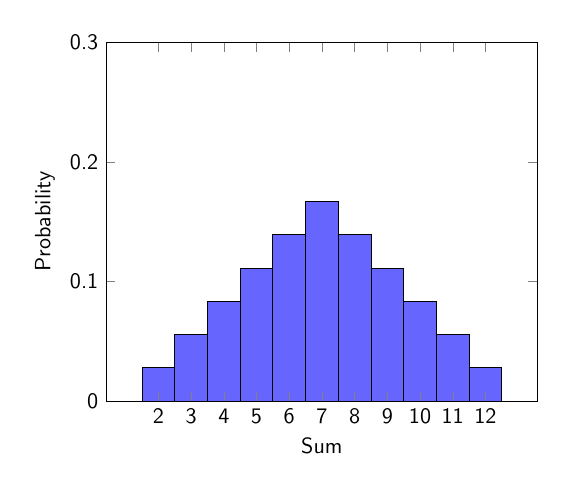
\begin{tikzpicture}[scale=0.8]
\begin{axis}[
ymin = 0, ymax = 0.3, area style, xlabel = {Sum}, ylabel = {Probability},
xtick = {2,3,...,12}
]
\addplot[ybar interval, fill=blue!60, mark=no] plot coordinates {
	(1.5,1/36) (2.5,1/18) (3.5,1/12) (4.5,1/9) (5.5,5/36) (6.5,1/6) (7.5,5/36) (8.5,1/9) (9.5,1/12) (10.5,1/18) (11.5,1/36) (12.5,1/36)
};
\end{axis}
\end{tikzpicture}
\end{center}


\begin{example}
\begin{enumerate}[(a)]
\item Create a probability distribution for flipping a coin three times, where $X$ represents the number of times heads is flipped.
\vspace{1.5in}
\item Create a probability distribution histogram for the number of times heads appears when flipping a coin 3 times.	
\end{enumerate}
\end{example}

\vspace{2.5in}

\begin{example}
The distribution below represents the percentage of households that have $x$ dogs according to a recent study. \newline
\begin{center}
\begin{tabular}{c|c}
$\pmb{x}$ & $\pmb{P(X=x)}$ \\ \hline
0 & 44\% \\
1 & 27\% \\
2 & 18\% \\
3 or more & 11\%
\end{tabular}
\end{center}
How many households have at least 1 dog?	
\end{example}

\subsection*{Expected Value of a Probability Distribution}


\begin{tcolorbox}[colframe=green!20!black, colback = green!30!white,title=\textbf{Expected Value}]
The \textbf{expected value} of a probability distribution is the outcome we would expect to happen if the experiment was performed a very large number of times.
\end{tcolorbox}
\vspace{10pt} 

In other words, it is a {\color{blue}\textbf{weighted mean}} of the distribution of outcomes:	
\[E(X) = \sum \left(x \cdot P(x)\right) \]

\vspace{2in}

\begin{example}
Determine the expected value of rolling two dice.
\end{example}

\vspace{1.5in}

\begin{example}
The distribution below represents the percentage of households that have $x$ dogs according to a recent study. \newline
\begin{center}
\begin{tabular}{c|c}
$\pmb{x}$ & $\pmb{P(X=x)}$ \\ \hline
0 & 44\% \\
1 & 27\% \\
2 & 18\% \\
3 & 11\%
\end{tabular}
\end{center}
What is the expected number of dogs per household?
\end{example}

\newpage 

\subsection*{Variance and Standard Deviation of a Probability Distribution}

Recall that 
\begin{itemize}
    \item {\color{blue}\textbf{Variance}} is the average squared deviation from the mean.
    \item {\color{blue}\textbf{Standard deviation}} is the square root of variance.
\end{itemize}

\vspace{0.25in}

With probability distributions, the {\color{blue}\textbf{mean}} is the {\color{orange}\textbf{expected value}}.

\vspace{0.5in}

\begin{center}
\setlength{\extrarowheight}{5pt}
\begin{tabular}{c|c|c}
    & \textbf{Variance} & \textbf{Standard Deviation} \\ \hline 
    \textbf{Typical Formula} & $\sigma^2 = \sum\left((x-\mu)^2 \cdot P(x)\right)$ & $\sigma = \sqrt{\sum\left((x-\mu)^2 \cdot P(x)\right)}$ \\[3pt] \hline 
    \textbf{Alternative Formula} & $\sigma^2 = \sum\left((x-E(x))^2 \cdot P(x)\right)$ & $\sigma = \sqrt{\sum\left((x-E(x))^2 \cdot P(x)\right)}$
\end{tabular}
\end{center}

\vspace{1in}

Fortunately, we will use technology for this. 

\vspace{1in}

\begin{example}
What is the standard deviation of rolling two dice?
\end{example}	

\vfill 

\begin{example}
Using the range rule of thumb, what are the minimum and maximum ``usual" values for rolling 2 dice?
\end{example}

\vfill 

\end{document}



